\chapter{Mezuro}

O Mezuro foi planejado para ser uma ferramenta de extração, análise e
interpretação de métricas de código-fonte. De uma forma geral, ele é dividido
em duas partes: para o processamento e para o cálculo é utilizado o Kalibro, que
é um \textit{webservice}; e o Prezento para a interface gráfica (uma aplicação
\textit{Web}) \cite{meirellesCibse2015}. Sob a licença
\textit{Affero General Public License version 3} (AGPLv3), o Mezuro permite que
o usuário crie, salve e edite ``configurações'' que são um conjunto de
métricas escolhidas por este e um ``grupo de leitura'' para provimento de uma
interface gráfica de um conjunto de leitura que tenha algum sentido quando
agrupadas, por exemplo: com a pontuação x, a métrica terá o ``rótulo'' ``BOM'' e
será atribuído a ela a cor amarela; com a pontuação x + 2, a métrica terá o
``rótulo'' ``ÓTIMO'' e estará com a cor verde. As cores são para destacar a
interpretação e são definidas com valores hexadecimal \cite{camarinhaOSS2015}.

Em 2013 o Mezuro foi totalmente reescrito em Ruby, com objetivo de manter na
mesma tecnologia as camadas da arquitetura. Mudança justificada também pela
necessidade do processamento dos cálculos e da análise. A carga de requisições,
mais a quantidade de núcleos que o servidor possuía, faziam com que a versão
original do Kalibro ficasse debilitado em seu fluxo de execuções. Outra vantagem
dessa reescrita é a facilidade com que novos contribuidores puderam/poderão
entender todo o funcionamento dessa parte do Mezuro. \cite{meirellesCibse2015}.

% Sobre o Prezento

A camada de apresentação do Mezuro é o Prezento, desenvolvido durante esse
processo de reescrita utilizando o \textit{framework} para desenvolvimento de
aplicações \textit{Web} Ruby on
Rails\footnote{\url{http://guides.rubyonrails.org/getting_started.html}}.
%
É nesta camada que está o foco das análises feitas neste trabalho.

\section{Métricas de Código-Fonte}

% TODO: Falar um pouco mais sobre métricas

Para entender a plataforma Mezuro e usá-la adequandamente, deve-se compreender o que são métricas de código-fonte, que o seu monitoramento está ligado a avaliação da qualidade interna de um produto de software.

% TODO: falar sobre os coletores, de forma direta e já exemplificando com métricas de código-fonte.
% TODO: footnote com as configurações do Mezuro

Métricas de código estão ligadas ao desenvolvimento, planejamento, custos,
produtividade e qualidade do software. Existem dois grandes conjuntos delas:
métricas tradicionais e métricas de orientação a objetos. São métricas
tradicionais: métricas de tamanho (ex. Linhas de Código - LOC), métricas de
complexidade (ex. Complexidade Ciclomática), métricas manutenibilidade, dentre
outras (Tamanho Médio dos Módulos, Uso de Variável, Número de Funções, por
exemplo). E são métricas de orientação a objetos: métricas de classes (ex.
Encapsulamento dos Atributos), métricas de métodos (ex. Média de Complexidade
dos Métodos), métricas de acoplamento (ex. Acoplamento Aferente), métricas de
herança (ex. Medida de Polimorfismo) e métricas de sistema (ex. Reúso de
Classe) \cite{meirelles2013monitoramento}.

% TODO: falar as métricas que são analisadas pelo Mezuro de fato
% TODO: escrever sobre os ranges de métricas somente no momento em que eu falo
%       das Configurações de Métricas

\section{Arquitetura e principais funcionalidades do Mezuro}

% TODO: atualizar esta arquitetura

Em resumo, a arquitetura do Mezuro é composta por três serviços, como
demonstrado na Figura \ref{fig:mezuroNoosferoArch}.

\begin{figure}[!htb]
	\centering
    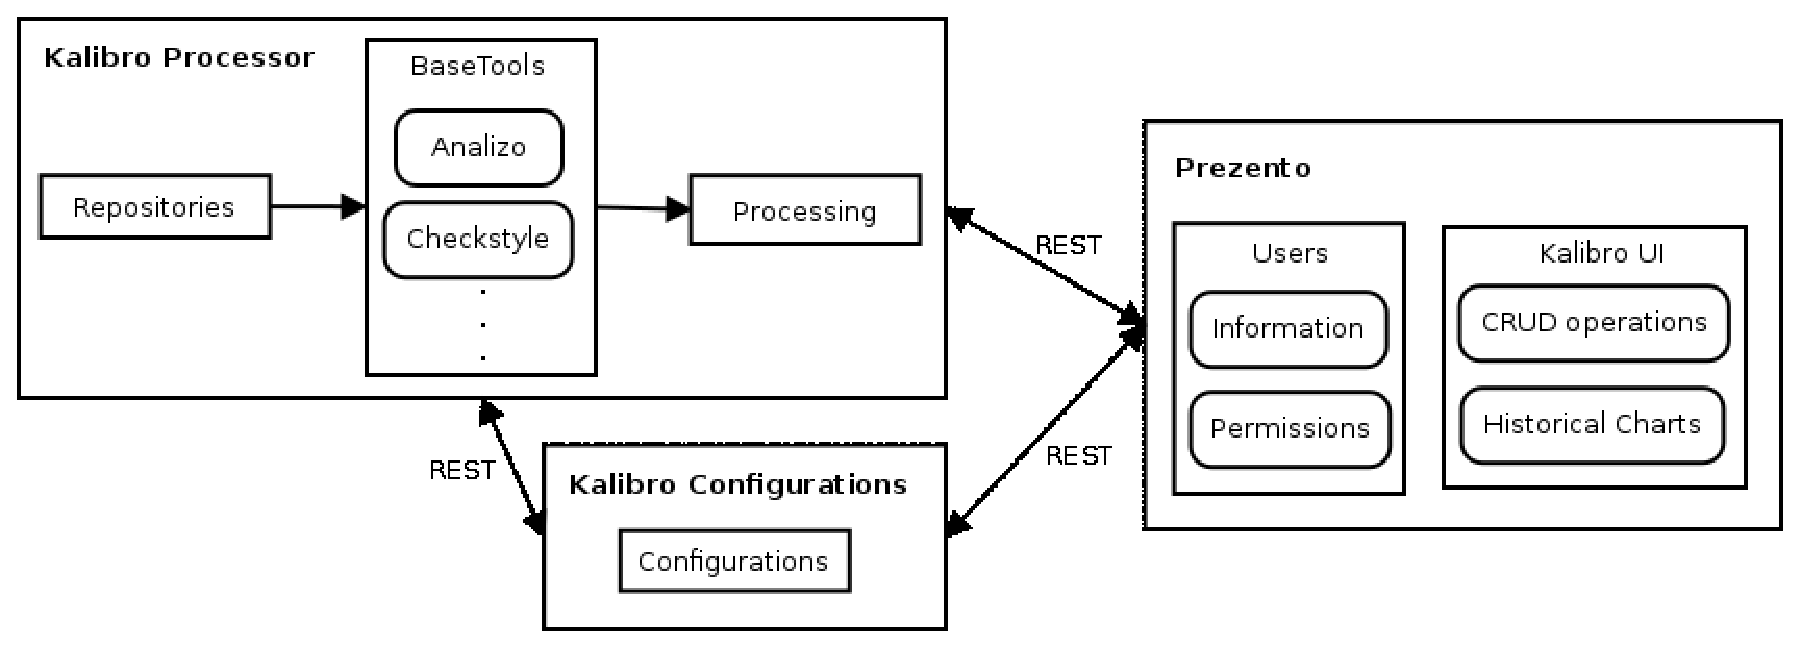
\includegraphics[keepaspectratio=true,scale=0.5]
    {figuras/mezuroCloudArch.eps}
  \caption{Arquitetura do Mezuro \cite{camarinhaOSS2015}}
	\label{fig:mezuroNoosferoArch}
\end{figure}

Onde os serviços são:

\begin{itemize}
  \item \textit{Prezento}: para a interface gráfica do usuário
  \item \textit{Kalibro Processor}: para a análise do código
  \item \textit{Kalibro Configurations}: para o gerenciamento das configurações
\end{itemize}

A decisão de dividir o Kalibro em serviços separados foi tomada para deixar
cada um deles com menos responsabilidades, facilitando a manutenção e evolução
\cite{camarinhaOSS2015}. E a comunicação entre estes serviços é feita através
do Kalibro Client: um quarto software também escrito em Ruby, mantendo a
escolha de centralização em uma única tecnologia. E, como demonstra Figura \ref{fig:mezuroNoosferoArch}, para simplificar a
implementação, também foi decidido que a comunicação entre os serviços seria
RESTful.

Dada essa arquitetura baseada em serviços, as principais funcionalidades podem ser
divididas em dois grupos:

\begin{itemize}
  \item Projeto
    \begin{itemize}
    \item \textit{Download} do código-fonte a partir de repositórios (Git,
    Subversion, Bazaar etc) ou via arquivo compactado;
        \item Escolha da periodicidade do processamento do código (1 dia, 2 dias,
        semanal, quinzenal e mensal);
        \item Escolha de qual configuração de métricas cada repositório irá
        utilizar;
        \item Nota de cada métrica da configuração para cada arquivo do
        repositório;
        \item Análise gráfica de cada arquivo do repositório por meio de um
        gráfico de pontos com notas ao longo do tempo;
        \item Resultados públicos e acessíveis à comunidade.
    \end{itemize}
    \item Configuração
    \begin{itemize}
    \item Criação de configuração e a possibilidade de clonagem;
        \item Estatísticas sobre as configurações mais populares dentro da
        comunidade;
        \item Criação de intervalos qualitativos associados aos valores das
        métricas;
        \item Criação de grupos de leitura para a interpretação textual dos
        resultados das métricas;
        \item Combinações de métricas nativas para criação de análises compostas
        e mais complexas.''
    \end{itemize}
\end{itemize}

\newpage

% TODO: com esse conjunto de funcionalidade o Mezuro apresenta-se como uma ferramenta
%       destaca-se portanto que o Mezuro é uma ferramenta com grande pontecial
%       em quem funcioliadades inovadoras e úteis, abordagem de interpretação adequada para o monitoramento, arquitetura bem modularizada,
%       por isso o foco deste trabalho em melhorar a camada de GUI, que é o prezento, para aproveitar este potencial

\section{Mezuro: Prezento}

O Prezento é a camada da interface web do
Mezuro. Desenvolvido em Ruby on Rails, atualmente utiliza as versões 2.3.0 do
Ruby e 4.2.4 do Rails. Versões estas que estão em constante mudança, pois os
autores têm como intuito usufruir o que há de mais recente das funcionalidades
dessa tecnologia. Esta será a principal camada trabalhada neste trabalho de
conclusão de curso, pois é nela que há a interação com o usuário.

% TODO: completar com mais infromações do Prezento e adicionar figuras de um Software do SPB.

% TODO: apresentar a navagabilidade e a apresentação dos resultados.
